\documentclass[conference]{IEEEtran}
\IEEEoverridecommandlockouts
% The preceding line is only needed to identify funding in the first footnote. If that is unneeded, please comment it out.
\usepackage{amssymb,amsmath,bm}
\usepackage{graphics,adjustbox}
\usepackage{tikz}
\usepackage{subfigure}
\usepackage{epstopdf}
\epstopdfsetup{suffix={}}
\usepackage{siunitx}
\sisetup{unitsep = \cdot}

\usepackage[figuresright]{rotating}
\usepackage[colorinlistoftodos]{todonotes}
\usepackage[english,algo2e,algoruled,vlined,linesnumbered]{algorithm2e}   % package for algorithm
\usepackage{enumerate}

\usepackage{easyReview}
\newtheorem{assumption}{Assumption}


\DeclareMathOperator*{\argmin}{arg min}

\def\BibTeX{{\rm B\kern-.05em{\sc i\kern-.025em b}\kern-.08em
    T\kern-.1667em\lower.7ex\hbox{E}\kern-.125emX}}
\begin{document}

\title{Model-free Reinforcement Learning Approach for Area Coverage Control using Heterogeneous Mobile Robots %
  %Model-free Reinforcement Learning Approach for Leader-Follower Formation Control Problems %
%  
% \thanks{This work was supported in part by the Bradley University’s Caterpillar fellowship grant.}
}

\author{%~
\IEEEauthorblockN{Amr Elhussein and Md Suruz Miah}
\IEEEauthorblockA{\textit{Electrical \& Computer Eng.} \\
\textit{Bradley University}, Peoria, Illinois, USA \\
aelhussein@mail.bradley.edu  and smiah@bradley.edu}
%\and
%\IEEEauthorblockN{Fazel Keshtkar}
%\IEEEauthorblockA{\textit{Div. of Computer Science, Math. and Science} \\
%\textit{St John's University}, Queens, NY, USA \\
%keshtkaf@stjohns.edu}
%\and
%\IEEEauthorblockN{Mohammed Abouheaf}
%\IEEEauthorblockA{\textit{School of EECS} \\
%\textit{Univ. of Ottawa}, Canada\\
%mabouhea@uottawa.ca}
%
}

\maketitle

\begin{abstract}
  %
In this paper, we present a novel model-free reinforcement learning approach for solving a conventional leader-follower problem using autonomous wheeled mobile robots. Specifically, the proposed learning approach decides the desired linear velocity and the steering angle (control actions) of a follower robot to follow the time-varying motion trajectory of
a leader robot. The setup of the online adaptive learning mechanism does not rely on any dynamical or kinematic information,~\textit{i.e.,} ``model-free'', of the car-like robots used in this work. Bellman's principle of optimality is employed to approximate the reward of the control actions determined by the proposed model-free adaptive learning algorithm. A set of computer experiments has been conducted to validate the performance of the proposed algorithm under various unplanned leader-trajectories. 
%
\end{abstract}

\begin{IEEEkeywords}
Leader-follower formation, mobile robots, reinforcement learning, policy iteration, trajectory tracking
\end{IEEEkeywords}

% \begin{nomenclature}
% \begin{deflist}[A]
% \defitem{ADP} \defterm{Approximate dynamic programming}
% \defitem{AL}\defterm{Approximate linearization}
% \defitem{RL}\defterm{Reinforcement learning}
% \end{deflist}
% \end{nomenclature}

\section{Introduction}
\label{sec:introduction}
The field of multi-agent systems %control theory 
is of a paramount importance in recent years due to its extensive applications in perimeter surveillance, search and rescue missions, cooperative localization, and target tracking tasks~\cite{Ma2019-Cooperative,Kia2018-ServerAssisted,Khan2018-Cooperative}. Multi-robot formation is one of many  active research topics within the realm of multi-agent systems and cooperative control theory~\cite{Oh2015-Survey}. In particular, the leader-follower problem has received thorough attention to the robotics community, where mobile robots follow leader robot(s) satisfying certain geometric constraints, such as cyclic pursuit~\cite{Yu2019-Cooperative,Marshall2004}, circular motion~\cite{Ma2019-Cooperative}, and time-varying communication topologies~\cite{Sakai208-Leader,Li2019-TimeVarying}. However,  many formation control strategies which are proposed in the literature to date rely on mathematical models of various mobile robots, such as underactuated autonomous surface vehicles~\cite{Liu2017-Modular}, nonholonomic wheeled mobile robots~\cite{Miao2018-Distributed}, unmanned underwater vehicles~\cite{Liu2019-Robust,Bechlioulis2019-Robust}, and unmanned helicopters~\cite{Kuo2019-Intelligent}.  In some cases, tools of computational intelligence are used to solve leader-follower problems, see~\cite{Xiao2019-LeaderFollower, Kuo2019-Intelligent}, for example, and some references therein, however, their learning mechanisms still rely on the underlying system dynamics. Recently, Miah~\textit{et~al.} developed several motion control strategies~\cite{MiKaCh2019-j1,MiKn2018-j1,MiFaChGu2017-j1,MiGu2015-j1,MiGu2014-j1} for nonholonomic mobile robots and fixed-base helicopters, where partial or full dynamical models are required for determining the desired control actions. 


The current manuscript overcomes some shortcomings associated with many leader-follower control approaches proposed in the literature by introducing an online model-free adaptive learning control mechanism. The proposed learning approach determines the actuator commands of a follower robot to follow an independent virtual leader. Note that the actuator commands (control actions) are the linear speed and steering angle of the follower robot. The learning mechanism relies on collecting the state information (i.e., position and orientation) of motion trajectories generated from both the leader and follower robots online over a finite time period. Bellman's principle of optimality is then formulated as a model-free reinforcement learning strategy to determine the optimal linear speed and the steering angle of the follower robot so that it follows the motion trajectories of the leader while maintaining a pre-defined safe distance between them. We emphasize that model parameters of both the leader and follower robots are unknown. Furthermore, the effectiveness of the proposed model-free reinforcement learning approach is validated by taking into consideration that the leader robot is a physical robot model as opposed to a simple point robot model, that is considered in many formation control, trajectory tracking, and leader-follower problems in the literature~\cite{Marshall2004}. 


% \emph{Notation:} Throughout this paper, sets will be denoted by caligraphic letters. For positive integers $m,n>0,$ $\mathbb{R}^n(\mathbb{R}^{m\times n})$ denotes a set of $n$--dimensional column vectors ($m\times n$-dimensional matrices) with entries taken from a set of real numbers $\mathbb{R}.$ Vectors (matrices) will be denoted with lowercase (uppercase) bold letters. A standard n-element column vector ${\bf x}$ will sometimes be represented as $[x_1,x_2,\ldots, x_n]^T$ with $[\cdot]^T$ being the transposition of the quantity $[\cdot].$ This allows to represent a column vector of vectors as $\mathbb{R}^{n^2}\ni{\bf v} = [{\bf x}_1,{\bf x}_2,\ldots,{\bf x}_n]^T.$ The standard Euclidean norm of the vector  ${\bf x}\in\mathbb{R}^n$ and the matrix ${\bf A}$ are given by $\Vert x \Vert = \left(\sum_{i=1}^n\lvert x_i\rvert^2\right)^{1/2}$ and $\Vert A \Vert = \left(\sum_{i=1}^m\sum_{j=1}^n\lvert a_{ij}\rvert^2\right)^{1/2}$  with $x_i,a_{ij}$ being the entries of ${\bf x}$ and ${\bf A},$ respectively. The scalar products of quantities ${\bf x},{\bf y}\in\mathbb{R}^n$ and ${\bf A}, {\bf B}\in\mathbb{R}^{m\times n},$ are given by %
% %
% \begin{align*}
%   {\bf x}^T{\bf y} = \sum_{i=1}^nx_iy_i~~\mathrm{and}~~{\bf A}\cdot {\bf B} =\mathrm{Tr}\left({\bf A}^T{\bf B}\right) = \mathrm{Tr}\left({\bf A}{\bf B}^T\right),
% \end{align*}
% %
% respectively, where $\mathrm{Tr}(\cdot)$ is the trace of matrix $(\cdot).$ Clearly, $\mathrm{Tr}({\bf A}^T{\bf A}) = \Vert {\bf A}\Vert^2.$ $\mathrm{diag}(a_1,a_2,\ldots, a_n)$ will denote an $n\times n$ diagonal matrix with elements $a_1,a_2,\ldots, a_n$ starting from its upper left corner. %

\section{Problem Setup} 
\label{sec:problemSetup}


Suppose that a car-like robot (follower) is deployed in a planar (2D) environment. Therefore, the coordinate $(x,y)$ is the position of the follower robot with an orientation of $\theta\in[-\pi,\pi)~\si{\radian}$ with respect to the global X-Y  coordinate frame.  Without loss of generality, the action commands of the robot are considered to be its linear speed $\nu$ and the steering angle $\gamma.$ Let ${\bf q}_k\equiv[x_k,y_k,\theta_k]^T$ denote the pose (position and orientation) vector of the robot at time $t\ge 0$ with $t=k \, T_s,$ $k\in\mathbb{N}_0,$ and $T_s>0$ being the sampling time.  The robot follows a leader trajectory defined by $(\mathbf{p}_k^{[\ell]})^T=[x_k^{[\ell]},y_k^{[\ell]}(t)]$ with the dynamics given in discrete-time as: %
%
\begin{align}
  \label{eq:leaderDT}
  \mathbf{p}_{k+1}^{[\ell]} = \mathbf{p}_k^{[\ell]} + T_s \, \mathbf{u}_k^{[\ell]},
\end{align}
%
where $\mathbf{u}_k^{[\ell]}\in\mathbb{R}^2$ is the control input vector of the leader at time instant $k,$ $k=0,1,\ldots.$ A standard setup of a leader-follower problem using car-like mobile robots is shown in Fig.~\ref{fig:leaderFollowerSetup}. The leader is supposed to maintain a constant safe distance $d>0.$
%
\begin{figure}
  \centering
  \fcolorbox{gray!10}{gray!5}{
    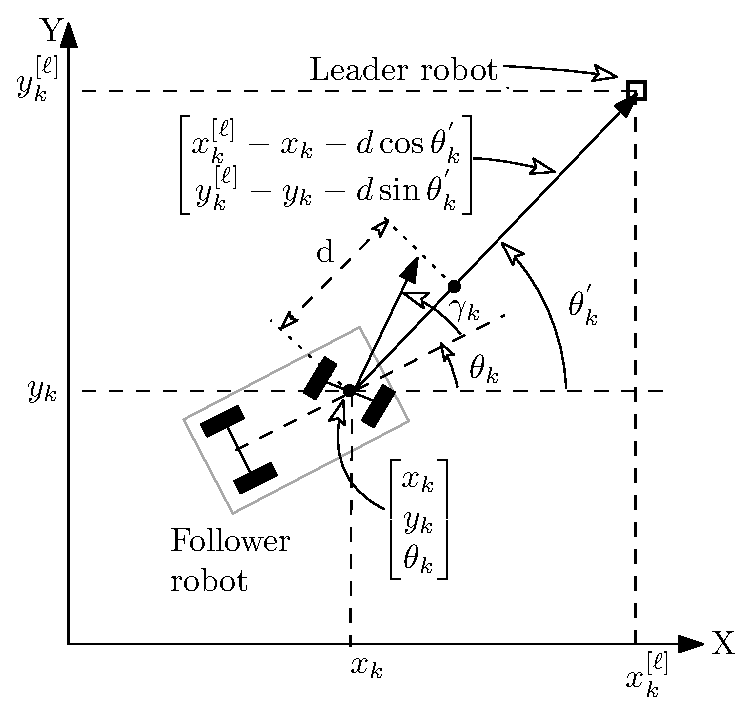
\includegraphics[width=0.45\textwidth]{figs/ipe/LF-Setup}
    }
  \caption{Mobile robot and its leader-follower problem setup.}
  \label{fig:leaderFollowerSetup}
\end{figure}
%
The robot's discrete-time model is approximated by the first-order Euler integration law given as: %
%
\begin{subequations}
  \begin{align}
    x_{k+1}& =x_{k}+T_s\nu_{k}\cos{(\theta_{k}+\gamma_{k})} + \zeta_1,\\  
    y_{k+1}& =y_{k}+T_s\nu_{k}\sin{(\theta_{k}+\gamma_{k})}+ \zeta_2,\\
    \theta_{k+1}&=\theta_{k}+T_s\nu_{k}\frac{\sin{(\gamma_{k})}}{l}+ \zeta_3,
  \end{align}
\label{eq:robotModel1-DT}
\end{subequations}
\\
where $\gamma_k\in(-\frac{\pi}{2},\frac{\pi}{2})$ is the front wheel steering angle with respect to the robot's orientation $\theta_k\in[-\pi,\pi),$ $\nu_k$ is the linear speed, $l$ is the distance between the drive wheels of the robot, and $\zeta_1,\zeta_2,\zeta_3\in\mathbb{R}$ are the model uncertainties. %
% A compact form of model~\eqref{eq:robotModel1-DT} can be written as %
% %
% \begin{align}
%   {\bf q}_{k+1} = {\bf q}_k + {\bf f}({\bf q}_k,{\bf u}_k,\bm{\zeta}_k),
%   \label{eq:robotModel1-DT1}
% \end{align}
% %
% where ${\bf f}:\mathbb{R}^3\times\mathbb{R}^2\times\mathbb{R}^3\to\mathbb{R}^3$ is a vector-valued vector function, ${\bf u}_k=[\nu_k,\gamma_k]^T\in\mathbb{R}^2$ is the robot's motion control input, and the model uncertainty vector is denoted by $\bm{\zeta}^T= [\zeta_1,\zeta_2,\zeta_3].$ %
%
It is assumed that, the left and right wheels of the robot steer together under a no-slip condition~\cite{Corke2011}. The state error between the follower and the leader is defined such that %
%
\begin{multline}
    \label{eq:stateError}
  \mathbf{e}_k^T = [x_e,y_e,\theta_e]^T = \\
  \begin{bmatrix}
    x_k^{[\ell]} - x_k - d\cos\theta_k^{'},
    y_k^{[\ell]} - y_k - d\sin\theta_k^{'},
    \theta_k^{'} - \theta_k
  \end{bmatrix},
\end{multline}
%
where $\theta_k^{'} = \mathrm{atan2}\left(y_k^{[\ell]}-y_k, x_k^{[\ell]}-x_k\right).$  %
%
The control problem can then be formally stated as follows: Find $\nu_k$ and $\gamma_k$ such that ${\bf e}_k\to {\bf 0}$ as  $k\to\infty$ subject to~\eqref{eq:leaderDT}~\text{and}~\eqref{eq:robotModel1-DT}. %
%     &\text{subject to}~\eqref{eq:leaderDT}~\text{and}~\eqref{eq:robotModel1-DT}.    %
% \begin{equation}
%   \begin{split}
%     &\mathrm{Find}~~\nu_k~\mathrm{and}~~\gamma_k~~\mathrm{such~that}\\
%     &{\bf e}_k\to {\bf 0}~~\mathrm{as}~ k\to\infty\\
%     &\text{subject to}~\eqref{eq:leaderDT}~\text{and}~\eqref{eq:robotModel1-DT}.    
%   \end{split}
%   \label{eq:problem}
% \end{equation}
%
The optimization goal is to let the follower robot asymptotically follow the leader robot while maintaining a safe distance $d>0$ regardless of motion trajectories with various complexities generated by the independent leader. It is emphasized that, the current model-free reinforcement learning mechanism determines  the control actions $\nu_k$ and $\gamma_k$ based on the error vectors $\mathbf{e}_k$ (data collected over a finite-time interval) as $k\to\infty.$ Before illustrating the proposed learning algorithm, let us briefly revisit the preliminaries of reinforcement learning in the next section. 


% In the next section, a conventional trajectory tracking method is investigated to solve the problem~\eqref{eq:problem}. This is followed by the proposed approximate dynamic programming technique which is illustrated in section~\ref{sec:solutionADP}.




\section{Preliminaries of Reinforcement Learning}
\label{sec:reinf-learn}
% greek letters: https://www.overleaf.com/learn/latex/List_of_Greek_letters_and_math_symbols

Reinforcement learning (RL) highlights a class of problems in the  field of multi-agent systems, where an agent determines sequential decisions (control actions) while learning from its associated environment. That is, an agent takes into account its learning  experience from the environment  and the cumulative reward to optimize decision~\cite{Francois-Lavet:2018}. The RL technology is described by four finite state tuples~$(\mathcal{S},\Omega,\mathcal{R},\mathcal{A}),$ that are  environment $(s \in \mathcal{S})$, agent $(w \in \Omega)$, reward $(r \in \mathcal{R})$, and action $(a \in \mathcal{A})$ as illustrated in Fig.~\ref{fig:fig-rl}. %
%
\begin{figure}
  \centering
  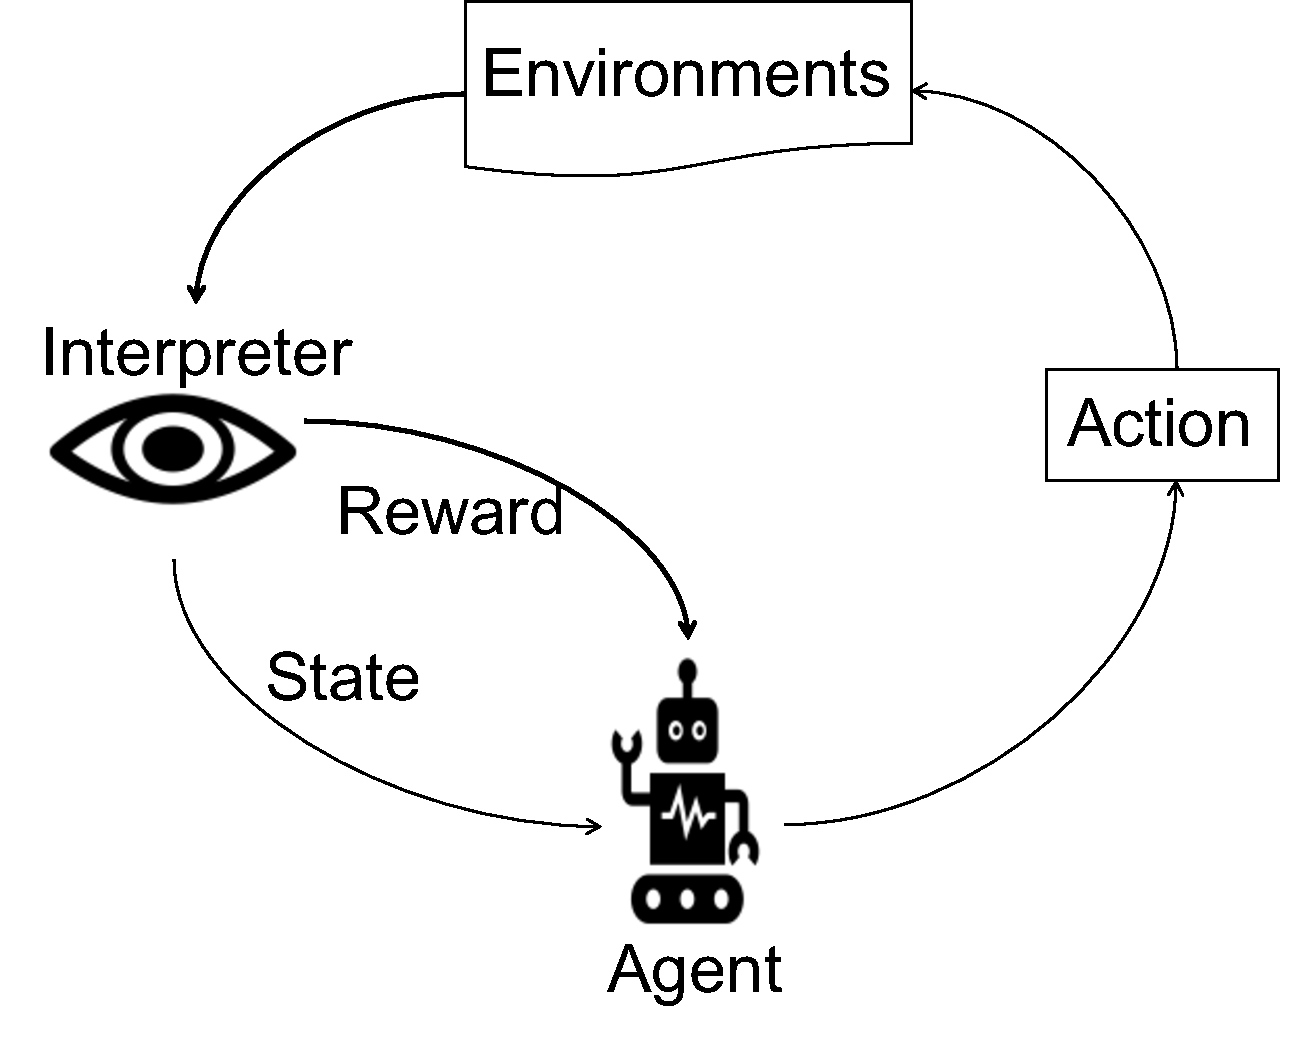
\includegraphics[scale=0.25]{figs/img/Ref-L-agent}
  \caption{A typical framing of a reinforcement learning scenario.}
  % \caption{A typical framing of a reinforcement learning scenario: an agent takes actions in an environment, which is interpreted into a reward and a representation of the state, which are fed back into the agent.}
  \label{fig:fig-rl}
\end{figure}
%
As pioneered by Barto~\textit{et al.} in~\cite{Barto1983-Neuronlike}, an agent determines its action in environment $s_0 \in \mathcal{S}$ by collecting information via agent $w_0 \in \Omega.$ Since the learning process is a sequential time based process, therefore, at each time step $k,$ an  agent determines  the action $a_k \in \mathcal{A}$ following three cascaded phases: (i) obtaining a reward $r_k \in \mathcal{R},$ % value function 
%
(ii) state transitions from agent state $s_k \in \mathcal{S}$ to $s_{k+1} \in \mathcal{S},$ % robot's state transition 
and (iii) the agent obtains an observation $w_{k+1} \in \Omega.$ %(error data)
% To summary, an RL model contains a four finite states tuples, Environment, Agent, Action, and Reward: $(S,\Omega, A, R)$. 
% \subsection{Our Reinforcement Learning Model} %
%
The leader-follower problem addressed in this paper is formulated using a model-free reinforcement learning approach as follows: %
%
%
%We defined and formulated the problem in mathematical models in section~\ref{sec:problemSetup}. To formulate RL for our problem, we define the four tuples as following:
\begin{enumerate}
    \item \textbf{Environment}: It is a 2D planar space where agents (leader and follower) interact with each other.
    \item \textbf{Agent}: Agents considered in this work are two robots (leader robot and follower robot). The robot motion behaviors are modeled using models~\eqref{eq:leaderDT}~and~\eqref{eq:robotModel1-DT}. The follower robot mimics the behavior of the leader robot. %The only information that follower robots received from the leader robot are its speed and steering angle.
    \item \textbf{Action}: The actions are the linear velocity and steering angles of the follower robot. Robots' state-transition task is performed using the control actions applied to their actuators. The main parameters that agents use to interact with the operating environment are the current position and orientation, speed, steering angle, and distance between the robots. 
    \item \textbf{Reward}: The goal here is to determine how follower robot can learn the leader robot's behavior to keep the minimum distance at any time and location to adjust its speed and distance. Therefore, follower robot will obtain reward $r_k \in \mathcal{R}$ at time instant $k$ if the distance between the follower and the leader is close to a safe distance $d.$ Herein, robots' state error is formulated as in \eqref{eq:robotModel1-DT}. Hence, once the error $\|\mathbf{e}_k\|$ is minimized at time instant $k,$ the follower robot will obtain reward $V,$ which is a modeled solving value function. This will be detailed out in the following section.
\end{enumerate}






\section{Proposed Model-Free RL Approach}
\label{sec:RLSolution}

The solution of the leader-follower formation problem is realized using a reinforcement learning approach. It employs model-free strategies for solving a temporal difference equation developed herein. This solution is equivalent to solving the underlying Bellman optimality equation for  the dynamical error model~\eqref{eq:stateError}. The relative importance of the states in the error vector ${\bf e}_k$ and the control decisions (linear velocity and steering angle) of the follower-robot are evaluated using the  performance (cost) index: %
\begin{align}
\label{eq:costFunctional}
J = \sum_{k=0}^\infty \frac{1}{2}\left[{\bf e}_k^T \, {\bf Q} \, {\bf e}_k + {\bf u}_k^T \, {\bf R} \, {\bf u_k}\right],
\end{align}    
where ${\bf Q}\in\mathbb{R}^{3\times 3}$ and ${\bf R}\in\mathbb{R}^{2\times 2}$ are symmetric positive definite weighting matrices. The objective of the optimization problem, following~\cite{Lewis2013-Reinforcement}, is to find an optimal sequence of control polices $\{\mathbf{u}^*_k\}_{k=0}^\infty$ that minimizes the cost index $J$ along the state-trajectories~\eqref{eq:leaderDT}~and~\eqref{eq:robotModel1-DT}. Motivated by the structure of the convex quadratic cost functional~\eqref{eq:costFunctional}, let the solution of the tracking control problem employ the value function $V({\bf e}_k,{\bf u}_k)$ defined by %
%
\begin{equation*}
\label{eq:valueFunction}
V({\bf e}_k,{\bf u}_k) = \sum_{\kappa=k}^\infty \frac{1}{2}\left({\bf e}_\kappa^T\, {\bf Q}\, {\bf e}_\kappa + {\bf u}_\kappa^T \, {\bf R}\, {\bf u_\kappa}\right).
\end{equation*}
%
This structure yields a temporal difference form (i.e., Bellman equation) as follows
\begin{equation*}
\label{eq:tempraldiffeq}
V({\bf e}_k,{\bf u}_k)= \frac{1}{2}\left[{\bf e}_k^T\, {\bf Q}\, {\bf e}_k + {\bf u}_k^T\, {\bf R}\, {\bf u_k}\right] +V({\bf e}_{k+1},{\bf u}_{k+1}).
\end{equation*}
%
Applying Bellman's optimality principle yields the optimal control policies ${\bf u}_k^*,~k\ge 0,$ such that~\cite{Lewis2012} %
%
\begin{align*}
{\bf u}^*_k = \argmin_{{\bf u}_k}\left[\frac{1}{2}\left[{\bf e}^T_k\,  {\bf Q}\, {\bf e}_k +{\bf u}^T_k\,  {\bf R} \,  {\bf u}_k\right]   +
V({\bf e}_{k+1},{\bf u}_{k+1})\right].
\label{eq:argMinControlAction}
\end{align*}
%
Alternatively, this optimal  policy form is equivalent to ${\bf u}^*_k = \argmin_{{\bf u}_k}\left[
V({\bf e}_{k},{\bf u}_{k})\right].$
Therefore, the underlying Bellman optimality equation follows %
%
\begin{equation*}
\label{eq:BellOpt}
V^*({\bf e}_k,{\bf u}^*_k)= \frac{1}{2}\left[{\bf e}_k^T\, {\bf Q}\, {\bf e}_k + {\bf u}_k^{*T}\, {\bf R}\, {\bf u}^*_k\right] +V^*({\bf e}_{k+1},{\bf u}^*_{k+1}),
\end{equation*}
%
where $V^*(\cdot,\cdot)$ is the optimal solution for Bellman optimality equation. This temporal difference equation is utilized by reinforcement learning process which solves the following temporal difference approximation form %
%
\begin{align}
\hat{V}(\mathbf{z}_k) = \frac{1}{2}\mathbf{z}_k^T\, \bar{\mathbf{P}}\, \mathbf{z}_k + \hat{V}(\mathbf{z}_{k+1}),
\label{eq:valueFunctionEstimated}
\end{align}
%
where $\mathbf{z}_k = \left[\mathbf{e}_k ,\mathbf{u}_k\right]^T\in\mathbb{R}^5,$ $V\left(\mathbf{e}_k,\mathbf{u}_k\right) \approx \hat{V}(\mathbf{z}_k),$  and $\bar{\mathbf{P}}$ is a symmetric block-diagonal matrix formed using $(\mathbf{Q},\mathbf{R}),$~\textit{i.e.,~}$\bar{\mathbf{P}} = \mathrm{blockdiag}(\mathbf{Q},\mathbf{R}).$ %
The approximation of the solving value function $\hat{V}(\mathbf{z}_k)$ employs a quadratic form so that $\hat{V}(\mathbf{z}_k)=\frac{1}{2}\mathbf{z}_k^T\, \mathbf{P}\, \mathbf{z}_k,$ where $\mathbf{P}\in\mathbb{R}^{5\times 5}$ is a positive definite matrix. Hence, the optimal control strategy $\mathbf{u}_k^*$ can be expressed as follows %
%
\begin{align}
\label{eq:modelFreePolicy}    
\mathbf{u}_k^* = \argmin_{\mathbf{u}_k}\left[\hat{V}(\mathbf{z}_k)\right] = -\,  \mathbf{P}_{uu}^{-1}\, \mathbf{P}_{ue}\, \mathbf{e}_k,
\end{align}
%
where $\mathbf{P}_{uu}$ and $\mathbf{P}_{ue}$ are sub-blocks of symmetric matrix $\mathbf{P}.$ %   
%

A two-step solution mechanism that is based on policy iteration is employed to solve the temporal difference equation~\eqref{eq:valueFunctionEstimated} using the policy~\eqref{eq:modelFreePolicy}. First, the adaptive critics are used to approximate the solving value function $\hat V(\cdot)$ using a multi-layer critic neural network as shown in Fig.~\ref{fig:nnCritic}. %
%
\begin{figure}
    \centering
    \fcolorbox{blue}{gray!5}{
        \begin{adjustbox}{max width = 0.45\textwidth}
            \tikzset{%
                input neuron/.style={
                    circle,
                    fill=green!50,
                    minimum size=0.7cm
                },
                neuron missing/.style={
                    draw=none, 
                    scale=1,
                    fill=white,
                    text height=0.01cm,
                    execute at begin node=\color{black}$\vdots$
                },
            }
            
            \tikzset{%
                hidden neuron/.style={
                    circle,
                    fill=blue!50,
                    minimum size=0.7cm
                },
                neuron missing/.style={
                    draw=none, 
                    scale=1,
                    fill=white,
                    text height=0.01cm,
                    execute at begin node=\color{black}$\vdots$
                },
            }
            
            \tikzset{%
                output neuron/.style={
                    circle,
                    fill=red!50,
                    minimum size=0.7cm
                },
                neuron missing/.style={
                    draw=none, 
                    scale=1,
                    fill=white,
                    text height=0.01cm,
                    execute at begin node=\color{black}$\vdots$
                },
            }
            
            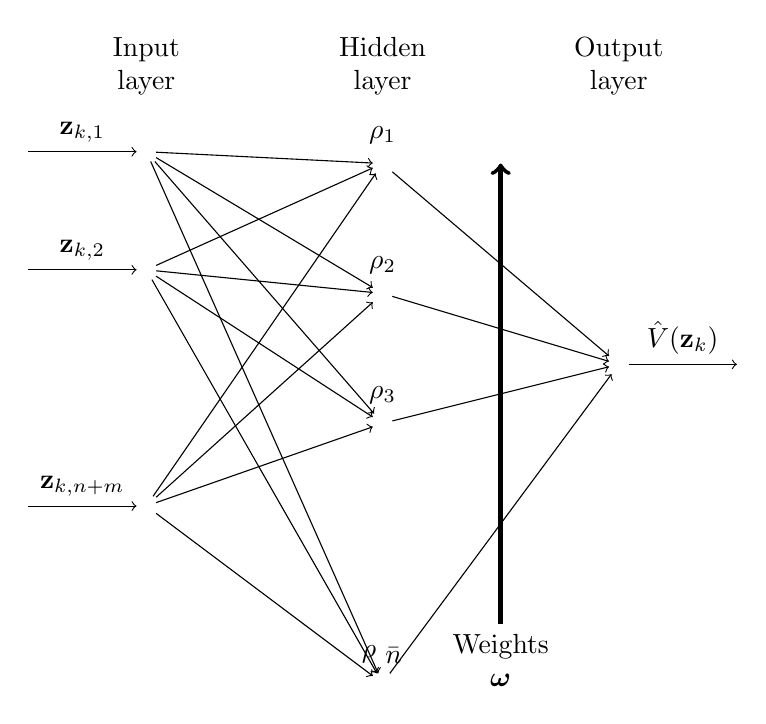
\begin{tikzpicture}[x=1.5cm, y=1.5cm]
            
            \foreach \m/\l [count=\y] in {1,2,missing,3}
            \node [input neuron/.try, neuron \m/.try] (input-\m) at (0,2.5-\y) {};
            
            \foreach \m [count=\y] in {1,2,3,missing,4}
            \node [hidden neuron/.try, neuron \m/.try ] (hidden-\m) at (2,2.5-\y*1.1) {};
            
            \foreach \m [count=\y] in {1}
            \node [output neuron/.try, neuron \m/.try] (output-\m) at (4,2.5-\y*2.8) {};
            
            \foreach \l [count=\i] in {1,2,n+m}
            \draw [<-] (input-\i) -- ++(-1,0)
            node [above, midway] {$\mathbf{z}_{k,\l}$};
            
            \foreach \l [count=\i] in {1,2,3,~\mbox{$\bar{n}$}}
            \node [above] at (hidden-\i.north) {$\rho_{\l}$};
            
            \foreach \l [count=\i] in {1}
            \draw [->] (output-\i) -- ++(1,0)
            node [above, midway] {$\hat{V}(\mathbf{z}_{k})$};
            % node [above, midway] {$\hat{V}_\l$};
            
            \foreach \i in {1,...,3}
            \foreach \j in {1,...,4}
            \draw [->] (input-\i) -- (hidden-\j);
            
            \foreach \i in {1,...,4}
            \foreach \j in {1}
            \draw [->] (hidden-\i) -- (output-\j);
            
            
            
            \foreach \l [count=\x from 0] in {Input, Hidden, Output}
            \node [align=center, above] at (\x*2,1.9) {\l \\ layer};
            
            \node [align=center, below] at (3,-2.5) {Weights \\ $\boldsymbol{\omega}$};
            \draw[->,ultra thick](3,-2.5) -- (3,1.4);
            
            \end{tikzpicture}
        \end{adjustbox}      
    }
    \caption{Critic neural network structure for approximating value function.}
    \label{fig:nnCritic}
      \end{figure}
%      
Second, the policy evaluation step of this process updates the critic weights $\bm{\omega}$ in real-time without acquiring any formation about the dynamics of the leader or follower dynamical systems  (the calculation mechanism of the critic weighs $\boldsymbol{\omega}$ is explained later on). This is done to search for a strictly better policy. %
%

Note that, the policy iteration computational setup rearranges the temporal difference expression~\eqref{eq:valueFunctionEstimated} such that %
%
\begin{equation}
\label{eq:const}
\mathbf{z}_k^T\, \mathbf{P}\, \mathbf{z}_k - \mathbf{z}_{k+1}^T\, \mathbf{P}\, \mathbf{z}_{k+1} = \mathbf{z}_k^T\, \bar{\mathbf{P}}\, \mathbf{z}_k. 
\end{equation}
%
This equation is utilized repeatedly in order to evaluate a certain policy during at least $\eta\ge \bar n, \bar n= (3+2)(3+2+1)/2$ evaluation steps (i.e., the lowest evaluation interval spans $k$ to $k+\bar n$ calculation samples) in order to update the critic weights vector  $\boldsymbol{\omega}=\mathrm{vec}(\mathbf{P}),$ which consists of connection weights between the neurons of the hidden layer and the output layer of the critic neural network shown in Fig.~\eqref{fig:nnCritic}. The operator $\mathrm{vec}(\mathbf{P})$ forms the columns of the $\mathbf{P}$ matrix into a column vector $\mathbf{\omega}$ of dimension $\bar{n}=15$ since the matrix $\mathbf{P}$ is a symmetric matrix. The left hand side of~\eqref{eq:const} is expressed using the following critic approximation form %
%
$$\hat{V}(\mathbf{z}_k)-\hat{V}(\mathbf{z}_{k+1})=\boldsymbol{\omega}^T\tilde{\bm{\rho}}(\mathbf{z}_{k,k+1}),$$
%
where $\tilde{\bm{\rho}}(\mathbf{z}_{k,k+1})=\bm{\rho}(\mathbf{z}_k)-\bm{\rho}(\mathbf{z}_{k+1}) \in \mathbb{R}^{15 \times 1}, \, \bm{\rho}(\mathbf{z}_k)=\left(\mathbf{z}^q_k\otimes\mathbf{z}^h_k\right)$ $(q=1,\dots, 5, \,\, h=q,\dots,5),$ and $\boldsymbol{\omega}^T = [0.5 \, P^{11},P^{12},P^{13},P^{14}, P^{15}, \, 0.5 \, P^{22}, P^{23},P^{24},P^{25},$ $\,0.5 \, P^{33}, P^{34},P^{35},\,0.5 \, P^{44},P^{45}, \,0.5 \, P^{55}]^T \in \mathbb{R}^{1\times 15}$ ($P^{ij}$ is the $ij^{th}$ entry of matrix $\mathbf{P}$). %
%
The critic weights $\boldsymbol{\omega}$ are updated using a gradient descent approach, where the tuning error $\varepsilon_k$ at each computational instance $k$ follows $\varepsilon_k =\boldsymbol{\omega}^T\tilde{\bm{\rho}}(\mathbf{z}_{k,k+1})-{v}_k,$ where $v_\kappa = \frac{1}{2}\mathbf{z}_{k}^T \, \bar{\mathbf{P}} \, \mathbf{z}_{k}$. As detailed earlier, it is required to perform at least $\eta \ge \bar n$ evaluation steps before updating the critic weights $\boldsymbol{\omega}$ (i.e., finding the new improved policy). Hence, it is required to minimize the sum of square errors such that %
%
\begin{multline*}
  \delta_c =\sum_{\kappa=0}^{\eta-1}\frac{1}{2}(\boldsymbol{\omega}^T\tilde{\bm{\rho}}(\mathbf{z}_{k+\kappa,k+\kappa+1})-{v}_{k+\kappa})^2 = \frac{1}{2}\| \mathbf{v} - \bm{\Lambda}\bm{\omega}\|^2\\
  =\frac{1}{2}\left(\mathbf{v} - \bm{\Lambda}\bm{\omega}\right)^T \left(\mathbf{v} - \bm{\Lambda}\bm{\omega}\right), 
\end{multline*}
where $\bm{\Lambda} = [{\bf o}_0,{\bf o}_1,\ldots,{\bf o}_{\eta-1}]^T \in \mathbb{R}^{\eta\times 15}$ with ${\bf o}_\kappa = \tilde{\bm{\rho}}^T({\bf z}_{k+\kappa, k+\kappa+1}) \in \mathbb{R}^{1\times 15}$ and ${\bf v} =[v_0,v_1,\ldots,v_{\eta-1}]^T \in \mathbb{R}^{\eta}$ with $v_\kappa = \frac{1}{2}\mathbf{z}_{k+\kappa}^T \, \bar{\mathbf{P}} \, \mathbf{z}_{k+\kappa}$ for $\kappa = 0,1,\ldots, \eta-1$. %
Therefore, the update law of the critic weights using the gradient decent approach for at least $\bar n$ samples is given by %
\begin{multline}
  \bm{\omega}^{[r+1]} = \bm{\omega}^{[r]} - \ell_c\frac{\partial\delta_c}{\partial \bm{\omega}} = \bm{\omega}^{[r]} - \ell_c\left(-\bm{\Lambda}^T\mathbf{v} + \bm{\Lambda}^T \bm{\Lambda}\bm{\omega}^{[r]}\right)\\ 
=\bm{\omega}^{[r]} - \ell_c \bm{\Lambda}^T\left(\bm{\Lambda}\bm{\omega}^{[r]}-\mathbf{v}\right), 
\label{eq:criticWeights}
\end{multline}
%
where $0<\ell_c<1$ is a critic learning rate and $r$ is the  update index of the critic weights. 

The newly computed critic weights $\boldsymbol{\omega}$ are used to reconstruct the matrix ${\bf P}$ (i.e., updating the solving value function and hence calculating the associated policy) such that 
%
\begin{center}
${\bf P}=\begin{bmatrix} 
2\,\omega^{1}    & \omega^{2}      & \omega^{3}       & \omega^{4}       & \omega^{5} \\ 
\omega^{2}       &2\, \omega^{6}   & \omega^{7}       & \omega^{8}       & \omega^{9} \\
\omega^{3}       & \omega^{7}      &2\, \omega^{10}   & \omega^{11}      & \omega^{12} \\
\omega^{4}       & \omega^{8}      & \omega^{11}      & 2\,\omega^{13}   & \omega^{14} \\
\omega^{5}       & \omega^{9}      & \omega^{12}      & \omega^{14}      & 2\,\omega^{15}   
\end{bmatrix}\in \mathbb{R}^{5\times 5},$
\end{center}
%
where $\omega^{i}$ is the $i^{th}$ entry of the weight vector $\bm{\omega}.$ The complete policy iteration solution process for the leader-follower problem is detailed out in Algorithm \ref{alg:ModelFreeTracking}. %
%
\begin{algorithm2e}
    \caption{\label{alg:ModelFreeTracking} Model-free reinforcement learning using the policy iteration solution.}
    \DontPrintSemicolon
    \KwIn{Sampling-time $T_s,$ $\mathbf{Q},~\text{and}~\mathbf{R}$ }
    \KwOut{Error trajectory $\mathbf{e}_k,$ for $k=0,1,\ldots$}
    % \KwData{Map representation using occupancy grid technique}
    % \KwResult{output******************************}
    \Begin{
        $k=0, r = 0$ \tcc*[h]{Discrete time and policy indices}\;
        $\eta = (n+m)(n+m+1)/2$\;
        Initialize $\mathbf{P}^{[0]}$ \tcc*[h]{Positive definite}\;
                Set offset distance $d$\;
                Given approximate initial poses of leader and follower, compute $\mathbf{e}_0$ using error model~\eqref{eq:stateError}\;
                Compute follower's input $\mathbf{u}_0^{[0]}$ using policy~\eqref{eq:modelFreePolicy}\;
        \Repeat(\tcc*[h]{Main timing loop}){Tracking errors are zero}
        {
            Find $\mathbf{e}_{k+1}$ using~\eqref{eq:stateError}\;
            Compute policy $\mathbf{u}_{k+1}^{[r]}$ using~\eqref{eq:modelFreePolicy}\;
            %Evaluate and record Equation~\eqref{eq:modelFreeMatrixSolution}\;
            \If{[$(k+1)~\mathrm{modulo}~\eta]==0$ }
            {
                $r\leftarrow r+1$\tcc*[h]{Evaluate policy}\;
                Solve for the critic-weights $\bm{\omega}$ using~\eqref{eq:criticWeights}\;
                Construct matrix $\mathbf{P}^{[r]}$ using vector $\bm{\omega}$\;
%                \eIf{$\|\mathbf{P}^{[r]} - \mathbf{P}^{[r+1]}\|<\varepsilon$}{Set $\mathbf{u}_{k+1}^*\leftarrow\mathbf{u}_{k+1}^{[r]}$}{$k\leftarrow k+1$ }
            }
%        {
%                $k\leftarrow k+1$
%            }
        $k\leftarrow k+1$
        }
    }
\end{algorithm2e}    
    
    


  

\section{Computer Experiments and Results}
\label{sec:resultsExperiments}
In the sequel, computer experiments  are conducted to validate the performance of the proposed model-free adaptive learning algorithm in real-time. The results of computer experiments highlight the dynamics of the tracking errors and the convergence characteristics of the proposed algorithm (i.e., updating the critic weights). This will judge the ability of the follower robot to track independent motion trajectory of the leader robot under two different independent leader-motion trajectories. The computer experiments are realized using MATLAB simulation environment. The weighting matrices are set to $\mathbf{Q} = \mathrm{diag}[0.01,0.01,0.005]$ and $\mathbf{R} = \mathrm{diag}[10^{-6}, 10^{-6}].$ % 
% \[Q=0.001 
% \begin{bmatrix}
% 10       & 0   & 0\\
% 0       & 10   & 0\\
% 0       & 0   &5 \\
% \end{bmatrix},
% R=0.000001
% \begin{bmatrix}
% 1       & 0 \\
% 0       & 1 
% \end{bmatrix}.\]
The learning rate $\ell_c$ is set to  $0.0001$. The sampling time $T_s$ is set to $0.08 \sec.$ The desired distance offset between the leader and the follower is set to $ d = 0.5$ [m] for all scenarios.

In the first scenario, the leader trajectory motion is described by a unicycle model so that %
%
% \begin{align*}
$\dot x^{[\ell]}(t) = \nu^{[\ell]}(t)\cos\theta^{[\ell]}(t),$ %
$\dot y^{[\ell]}(t) = \nu^{[\ell]}(t)\sin\theta^{[\ell]}(t).$
%\dot\theta^\ell(t) &= \omega(t),
% \end{align*}
%
Initially, the leader's position is set to be the same for a short period of time with $\nu^{\ell} = 0 , \gamma^{\ell} = 0$. Then it starts to move on a horizontal line with $\nu^{\ell} = 0.1 $ [m/s], eventually the leader starts to move on an inclined path with $\nu^{\ell} = 0.2$ [m/s], $\gamma^{\ell} = 45\degree$. The leader is initially placed at $(x,y) = (5, 2)~\si{[\meter]}$ with an orientation of $\theta = 0 \degree $, while the follower  is initially placed at $(x,y) = (0, 0)~\si{[\meter]}$ with an orientation of $\theta = 0\degree$. Note that during this scenario, the critic weights converge rapidly and the tracking errors decay till the follower tracks the leader. The trajectory phase plan plot, tracking error states, control signals, and tuning of critic weights are shown in Fig.~\ref{fig:performanceRectilinearTrajectory}. %
%
\begin{figure*}[htbp]%
    \centering
    %\parbox[c]{0.48\textwidth}{\centering Parallel parking}
    %\parbox[c]{0.48\textwidth}{\centering Trajectory tracking}
    %\\
    \subfigure[][]{%
        \label{fig:trajectoryRectilinearDistance}%
        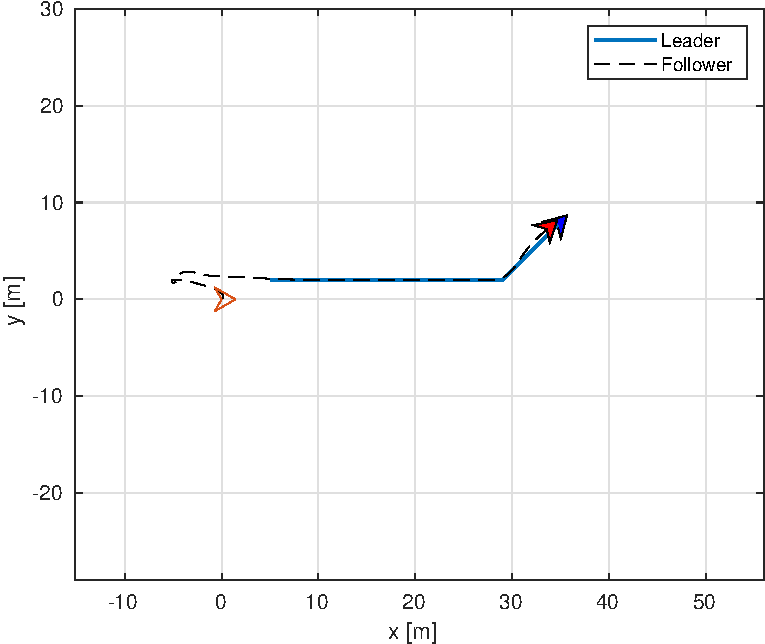
\includegraphics[width=0.48\textwidth,height=0.25\textheight]{figs/matlab/rectilinear/trajectoryRectlinearDistance} }
    \subfigure[][]{%
        \label{fig:stateErrorRectilinearDistance}%
        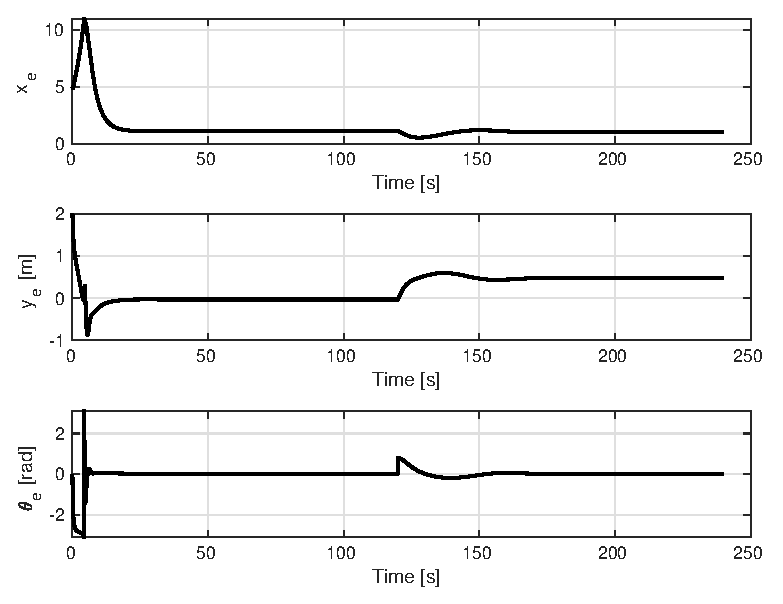
\includegraphics[width=0.48\textwidth,height=0.25\textheight]{figs/matlab/rectilinear/stateErrorRectlinearDistance} }
    \\
    \subfigure[][]{%
        \label{fig:controlInputsRectilinearDistance}%
        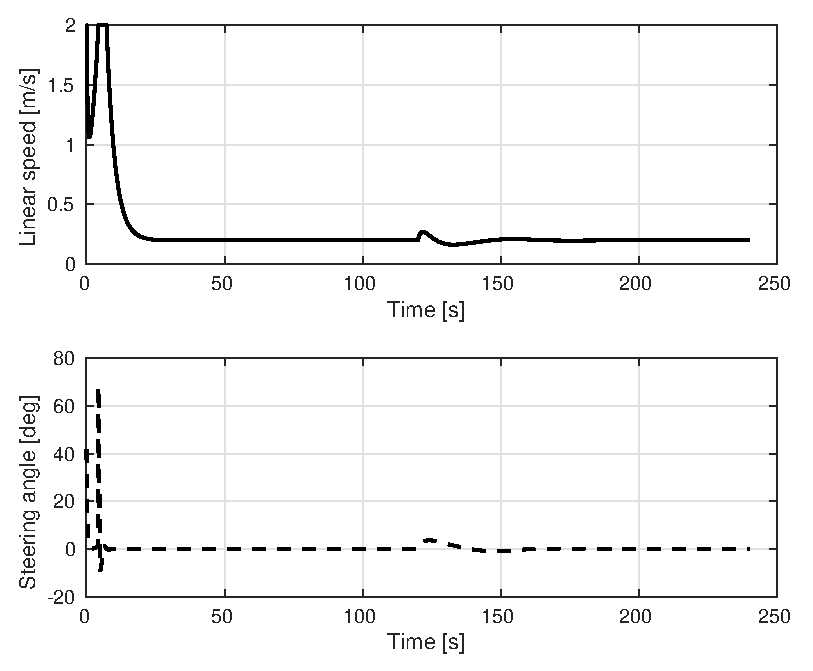
\includegraphics[width=0.48\textwidth,height=0.25\textheight]{figs/matlab/rectilinear/controlInputRectlinearDistance} }
    \subfigure[][]{%
        \label{fig:weightRectilinearDistance}%
        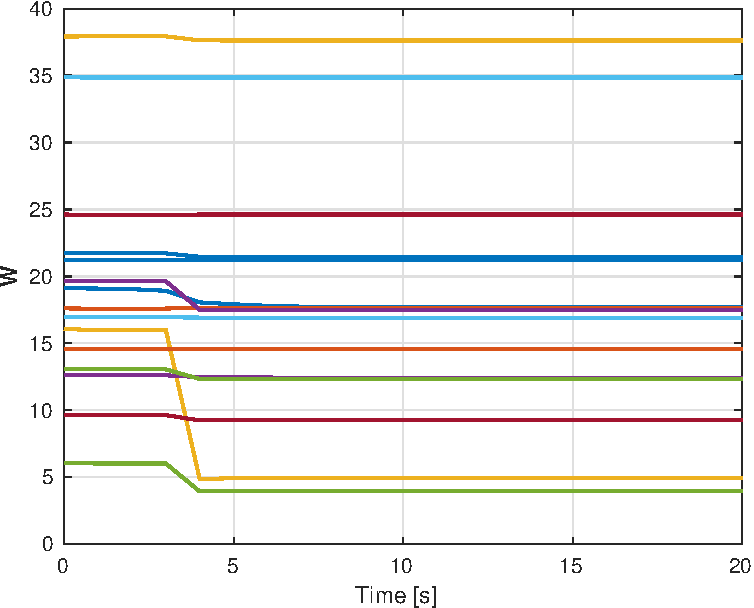
\includegraphics[width=0.48\textwidth,height=0.25\textheight]{figs/matlab/rectilinear/weightRectilinearDistance} }
    \caption[Leader-follower performance for rectilinear trajectory.]{First scenario (rectilinear trajectory): 
        \subref{fig:trajectoryRectilinearDistance} leader-follower trajectories,~\subref{fig:stateErrorRectilinearDistance} state tracking errors,~\subref{fig:controlInputsRectilinearDistance} linear speed and steering angle of the follower, and    \subref{fig:weightRectilinearDistance} critic weights.}%
    \label{fig:performanceRectilinearTrajectory}%
\end{figure*}
%


A relatively unplanned complex trajectory-tracking scenario is considered. The leader moves according to a sinusoidal trajectory so that %
%
% \begin{align*}
$x^{[\ell]}(t) = \alpha (t) \in [0,10\pi],$ %
$y^{[\ell]}(t) = 5 \,\sin(\alpha t),$ and %
$\theta^{[\ell]}(t) = cos(\alpha t).$  %
    %   \end{align*}
%
The leader robot  was initially placed at $(x,y) = (0, 0)~\si{[\meter]}$ with an orientation of $\theta = 0 \degree$ while the follower robot was initially placed at a random position around $(x,y) = (0, 0)~\si{[\meter]}$ with a random orientation. The simulation results are summarized in Figure~\ref{fig:performanceSinewaveTrajectory}. It is observed that the critic weights take more time to converge compared to the earlier scenario,  which is reluctant to the complexity of the independent trajectory of the leader. This result emphasizes the adaptability of the proposed adaptive learning mechanism to different scenarios. Further, the follower starts to move away from the leader at the beginning of the simulation before it finally converges to the leader where the tracking errors are bounded by a safe distance $d.$ % 
%
\begin{figure*}[htbp]%
    \centering
    %\parbox[c]{0.48\textwidth}{\centering Parallel parking}
    %\parbox[c]{0.48\textwidth}{\centering Trajectory tracking}
    %\\
    \subfigure[][]{%
        \label{fig:trajectorySinewave}%
        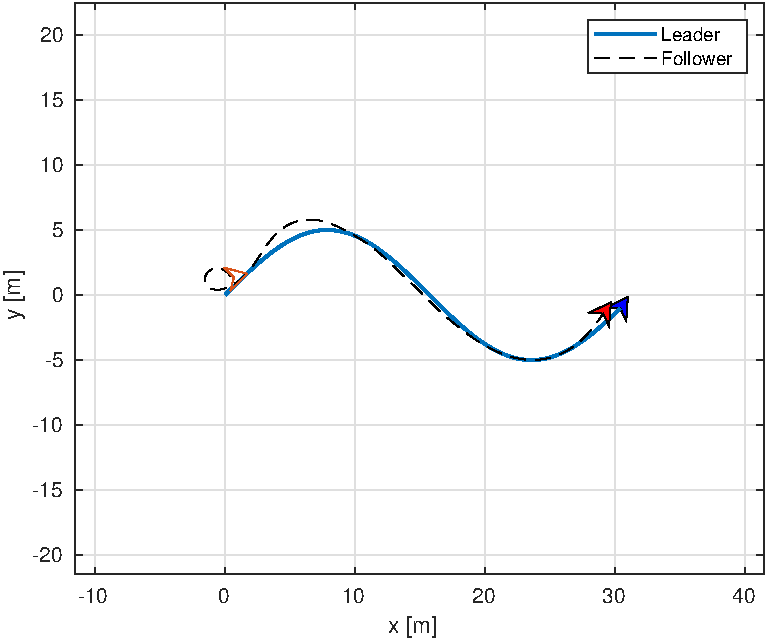
\includegraphics[width=0.48\textwidth,height=0.25\textheight]{figs/matlab/sinewave/trajectorySinewaveDistance} }
    \subfigure[][]{%
        \label{fig:stateErrorSinewave}%
        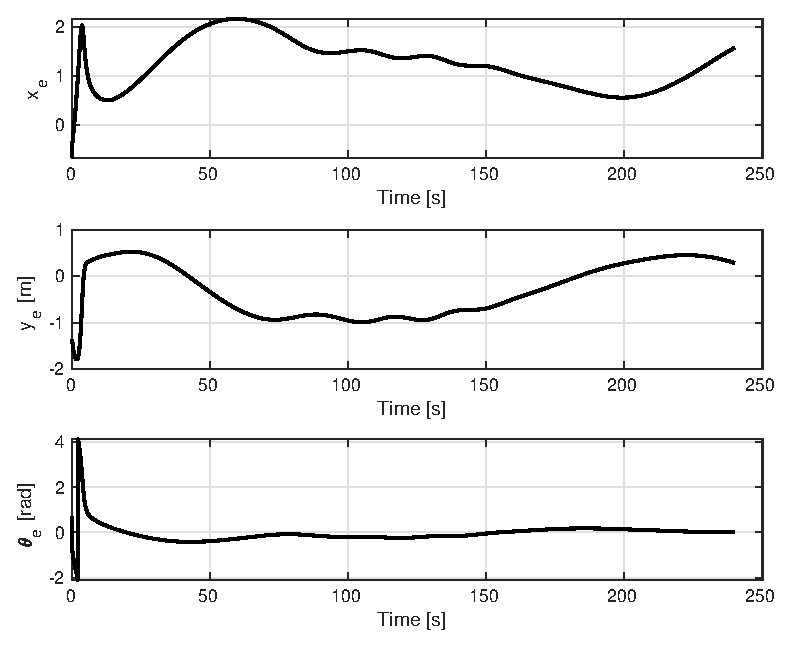
\includegraphics[width=0.48\textwidth,height=0.25\textheight]{figs/matlab/sinewave/stateErrorSinewaveDistance} }
    \\
    \subfigure[][]{%
        \label{fig:controlInputSinewave}%
        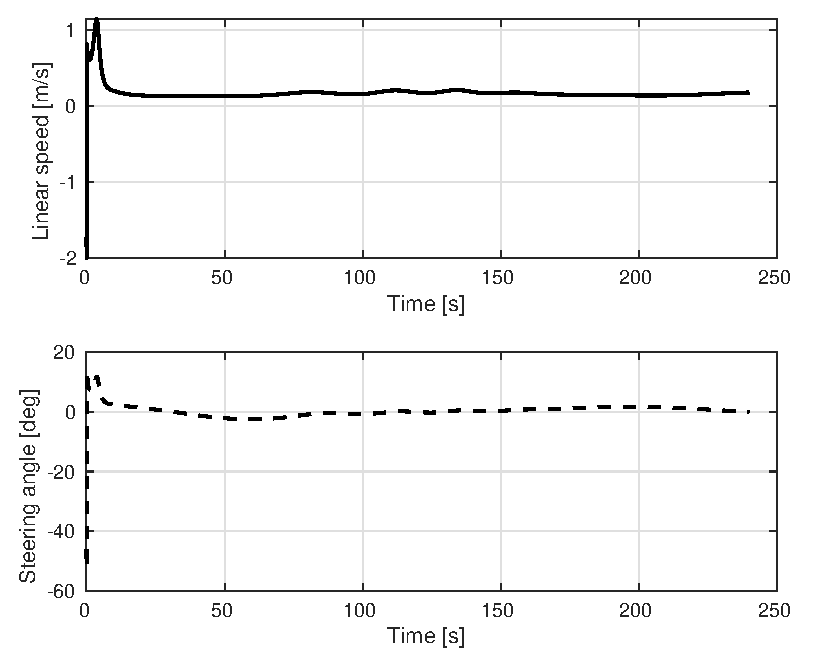
\includegraphics[width=0.48\textwidth,height=0.25\textheight]{figs/matlab/sinewave/controlInputSinewaveDistance} }
    \subfigure[][]{%
        \label{fig:weightSinewaveDistance}%
        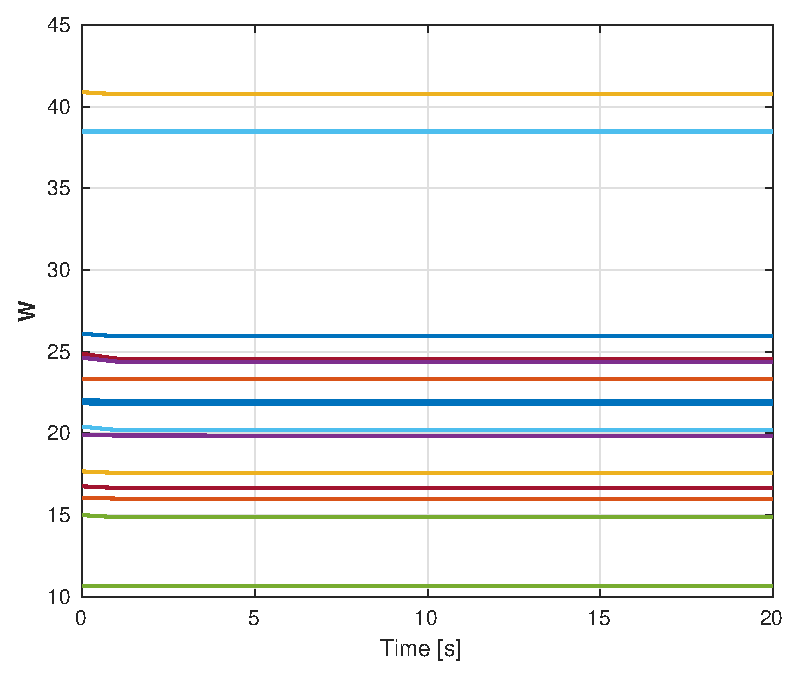
\includegraphics[width=0.48\textwidth,height=0.25\textheight]{figs/matlab/sinewave/weightSinewaveDistance} }
    \caption[Leader-follower performance for nonlinear trajectory.]{Second scenario (sinusoidal trajectory): 
        \subref{fig:trajectorySinewave} leader-follower trajectories,~\subref{fig:stateErrorSinewave} state tracking errors,~\subref{fig:controlInputSinewave} linear speed and steering angle of the follower, and    \subref{fig:weightSinewaveDistance} critic weights.}%
    \label{fig:performanceSinewaveTrajectory}%
\end{figure*}
%


%In the third case study we rely on completley random path for the leader robot to evaluate the effectivenss of the proposed algorithm as a solution for the leader follower tracking problem. The leader is to follow a random path defined by the model described in (2), with $\gamma$ being a random value, The follwer is to maitain an offset distance of $d = 0.5 $ [m]. Note that the path of the leader is not pre defined and the algorithm being completlety model free. The results are summerized in Fig. \ref{fig:peformanceRandomTrajectory}. %


%The results are summarized in Fig.~\ref{fig:peformanceRandomTrajectory}. %
%
%\begin{figure*}[htbp]%
%\centering
%%\parbox[c]{0.48\textwidth}{\centering Parallel parking}
%%\parbox[c]{0.48\textwidth}{\centering Trajectory tracking}
%%\\
%\subfigure[][]{%
%    \label{fig:trajectoryRandom}%
%    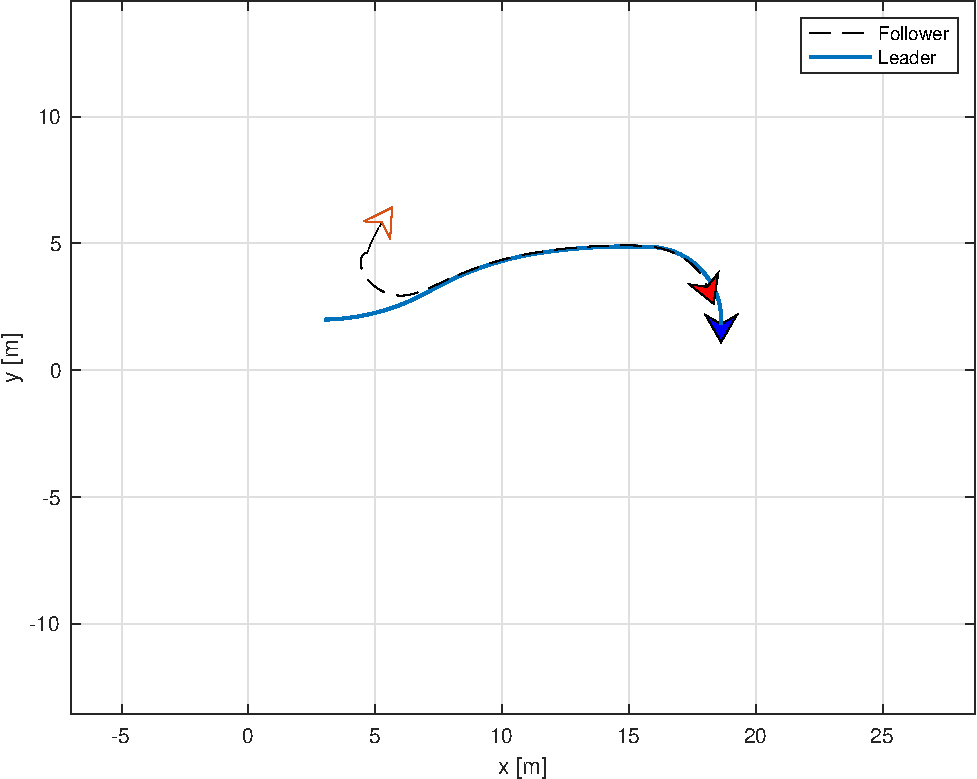
\includegraphics[width=0.48\textwidth,height=0.25\textheight]{figs/matlab/randomPath/trajectorySinewave} }
%\subfigure[][]{%
%    \label{fig:stateErrorRandom}%
%    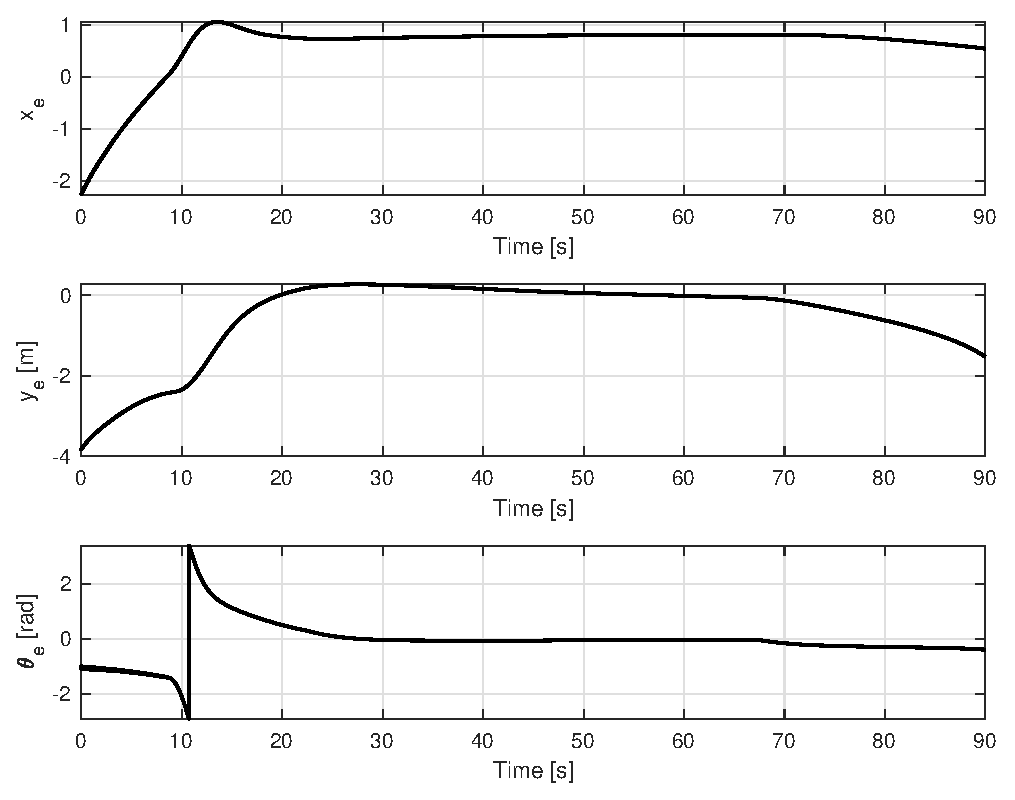
\includegraphics[width=0.48\textwidth,height=0.25\textheight]{figs/matlab/randomPath/stateErrorSinewave} }
%\\
% \subfigure[][]{%
%    \label{fig:controlInputsRandom}%
%    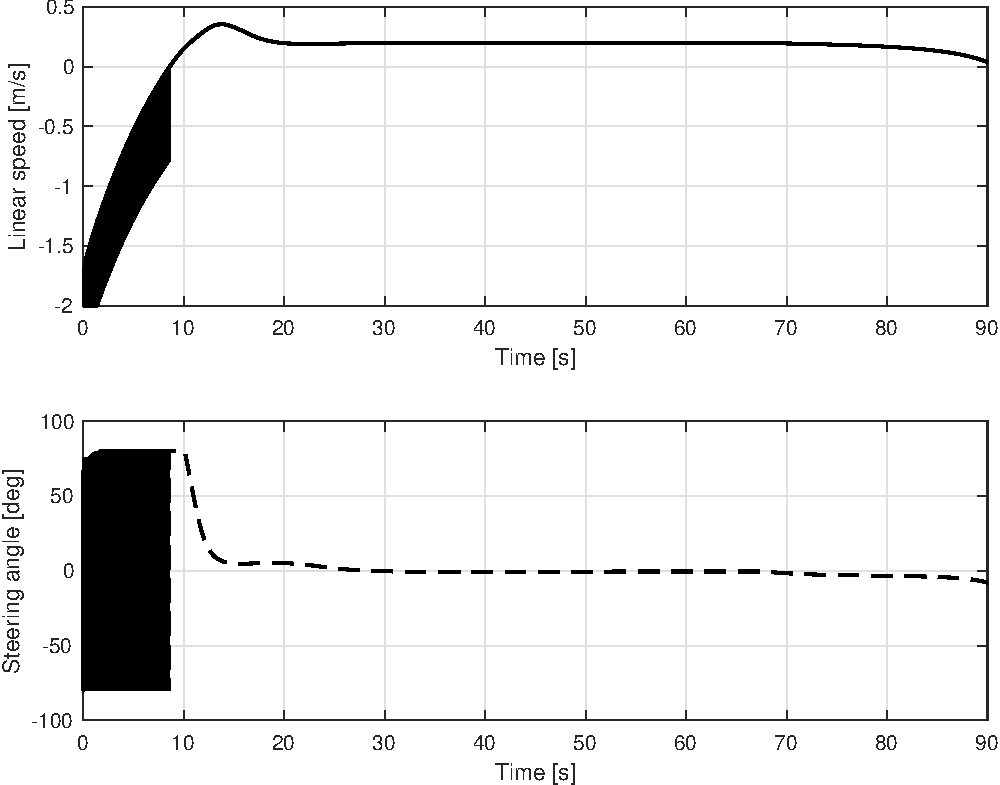
\includegraphics[width=0.48\textwidth,height=0.25\textheight]{figs/matlab/randomPath/controlInputSinewave} }
% \subfigure[][]{%
%    \label{fig:weightRandomDistance}%
%    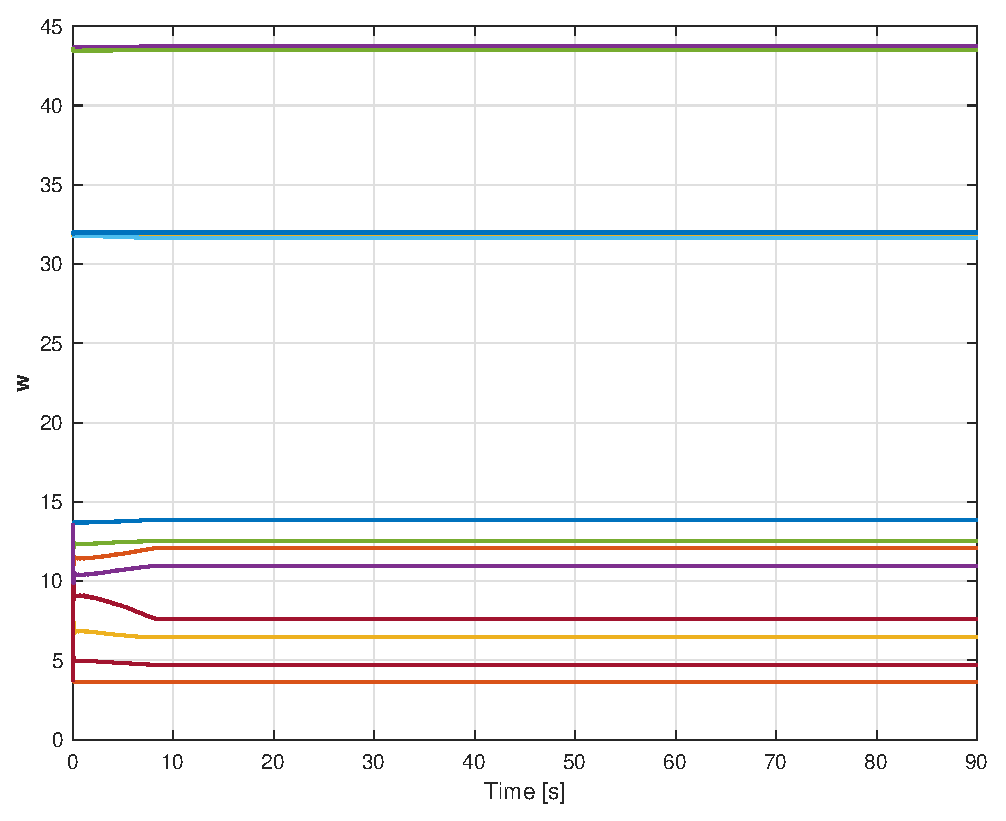
\includegraphics[width=0.48\textwidth,height=0.25\textheight]{figs/matlab/randomPath/weightRectilinearDistance} }
%\caption[Leader-follower performance for random trajectory.]{Performance in tracking random trajectory: 
%  \subref{fig:trajectoryRandom} leader-follower trajectories,~\subref{fig:stateErrorRandom} state error,~\subref{fig:controlInputsRandom} linear speed and steering angle of the follower; and    \subref{fig:weightRandomDistance} learning weights.}%
%  \label{fig:peformanceRandomTrajectory}%
%\end{figure*}
%


\section{Conclusion} \label{sec:conclusion}

A novel policy iteration mechanism based on a model-free reinforcement learning approach is presented for solving a conventional leader-follower formation problem using car-like mobile robots. The proposed approach does not rely on model parameters inherent in the mobile robots employed in this work. The follower robot is able to follow the leader robot that navigates along unplanned trajectories of various complexities while maintaining a nonzero safe distance between them. To the best of authors' knowledge, this is the first milestone of its kind where a model-free policy iteration based reinforcement learning approach is employed in a multi-robot formation control problem. The future work is going  to extend the learning algorithm for solving a time-varying formation control problem using networked robots.

% \section*{Acknowledgment}

% The preferred spelling of the word ``acknowledgment'' in America is without 
% an ``e'' after the ``g''. Avoid the stilted expression ``one of us (R. B. 
% G.) thanks $\ldots$''. Instead, try ``R. B. G. thanks$\ldots$''. Put sponsor 
% acknowledgments in the unnumbered footnote on the first page.



\bibliographystyle{IEEEtran}
\bibliography{bib/refsSuruzWeb,bib/refsMultiAgent,bib/refsRoboticsJournals,bib/refsRoboticsConferences,bib/refsGenericControl,bib/refsBooksTRTheses,bib/refsReinforcementLearningADP,bib/refsRL-Keshtkar}
\end{document}

%%% Local Variables:
%%% mode: latex
%%% TeX-master: t
%%% End:
